\chapter{Instant Insanity Puzzle}

Rishnak was examining the headstones of some graves and came across a headstone with a name Schossow\footnote{ Schossow got a patent for proposing this puzzle in 1899. \url{https://patents.google.com/patent/US646463A/en} }  in a grave. That brought him memories of the puzzle called the Great Tantalizer (also known as Instant Insanity). Schossow's puzzle had card suits (Hearts, Diamonds, Clubs and Spades) marked on each face. Frank Armbruster made a variation of this puzzle with colors instead of suits and that puzzle is called Instant Insanity Puzzle.
Rishnak thought this puzzle with a graph theoretic solution would appeal to Ajur. Soon after Rishnak spotted Ajur and Jura. Excitedly, Rishnak told Ajur that he wanted to talk about a puzzle which has a short solution using graph theory or a long solution using a search technique. The puzzle consists of four cubes with each face colored as shown in Figure \ref{22p1}. 
\begin{figure}
\begin{center}
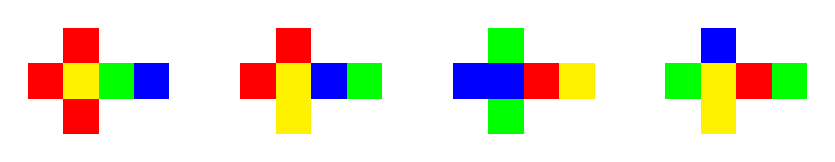
\begin{tikzpicture}
[scale=.9]
%First Cube
\fill [red] (0.0,0.0) rectangle (0.5,0.5);
\fill [yellow] (0.5,0.0) rectangle (1.0,0.5);
\fill [green] (1.0,0.0) rectangle (1.5,0.5);
\fill [blue] (1.5,0.0) rectangle (2.0,0.5);
\fill [red] (0.5,-0.5) rectangle (1.0,0.0);
\fill [red] (0.5,0.5) rectangle (1.0,1.0);
%Second Cube
\fill [red] (3.0,0.0) rectangle (3.5,0.5);
\fill [yellow] (3.5,0.0) rectangle (4.0,0.5);
\fill [blue] (4.0,0.0) rectangle (4.5,0.5);
\fill [green] (4.5,0.0) rectangle (5.0,0.5);
\fill [yellow] (3.5,-0.5) rectangle (4.0,0.0);
\fill [red] (3.5,0.5) rectangle (4.0,1.0);
%Third  Cube
\fill [blue] (6.0,0.0) rectangle (6.5,0.5);
\fill [blue] (6.5,0.0) rectangle (7.0,0.5);
\fill [red] (7.0,0.0) rectangle (7.5,0.5);
\fill [yellow] (7.5,0.0) rectangle (8.0,0.5);
\fill [green] (6.5,-0.5) rectangle (7.0,0.0);
\fill [green] (6.5,0.5) rectangle (7.0,1.0);
%Fourth Cube
\fill [green] (9.0,0.0) rectangle (9.5,0.5);
\fill [yellow] (9.5,0.0) rectangle (10.0,0.5);
\fill [red] (10.0,0.0) rectangle (10.5,0.5);
\fill [green] (10.5,0.0) rectangle (11.0,0.5);
\fill [yellow] (9.5,-0.5) rectangle (10.0,0.0);
\fill [blue] (9.5,0.5) rectangle (10.0,1.0);
\end{tikzpicture}
\caption{ Four Cubes}\label{22p1}
\end{center}
\end{figure}

The problem is to stack the four cubes vertically (in a column) so that all the cubes in each side (left, right, front and back) have distinct colors.
\begin{figure}
\begin{center}
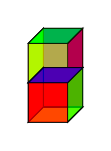
\begin{tikzpicture}
\coordinate (O) at (0,0,0);
\coordinate (A) at (0,0.5,0);
\coordinate (B) at (0,0.5,0.5);
\coordinate (C) at (0,0,0.5);
\coordinate (D) at (0.5,0,0);
\coordinate (E) at (0.5,0.5,0);
\coordinate (F) at (0.5,0.5,0.5);
\coordinate (G) at (0.5,0,0.5);

\draw[black,fill=yellow] (O) -- (C) -- (G) -- (D) -- cycle;% Bottom Face
\draw[black,fill=blue] (O) -- (A) -- (E) -- (D) -- cycle;% Back Face
\draw[black,fill=green] (O) -- (A) -- (B) -- (C) -- cycle;% Left Face
\draw[black,fill=red,opacity=0.7] (D) -- (E) -- (F) -- (G) --cycle;% Right Face
\draw[black,fill=yellow,opacity=0.7] (C) -- (B) -- (F) -- (G) --cycle;% Front Face
\draw[black,fill=green,opacity=0.7] (A) -- (B) -- (F) -- (E) -- cycle;% Top Face
\coordinate (OO) at (0,-0.5,0);
\coordinate (AA) at (0,0,0);
\coordinate (BB) at (0,0,0.5);
\coordinate (CC) at (0,-0.5,0.5);
\coordinate (DD) at (0.5,-0.5,0);
\coordinate (EE) at (0.5,0,0);
\coordinate (FF) at (0.5,0,0.5);
\coordinate (GG) at (0.5,-0.5,0.5);

\draw[black,fill=yellow] (OO) -- (CC) -- (GG) -- (DD) -- cycle;% Bottom Face
\draw[black,fill=red] (OO) -- (AA) -- (EE) -- (DD) -- cycle;% Back Face
\draw[black,fill=red] (OO) -- (AA) -- (BB) -- (CC) -- cycle;% Left Face
\draw[black,fill=green,opacity=0.7] (DD) -- (EE) -- (FF) -- (GG) --cycle;% Right Face
\draw[black,fill=red,opacity=0.7] (CC) -- (BB) -- (FF) -- (GG) --cycle;% Front Face
\draw[black,fill=blue,opacity=0.7] (AA) -- (BB) -- (FF) -- (EE) -- cycle;% Top Face
%% Following is for debugging purposes so you can see where the points are
%% These are last so that they show up on top
%\foreach \xy in {O, A, B, C, D, E, F, G}{
%    \node at (\xy) {\xy};
%}
\end{tikzpicture}
\caption{ Cube 4 on top of Cube 1 all faces have distinct colors}\label{22p2}
\end{center}
\end{figure}

We have illustrated with two cubes Cube number 4 sitting on top of Cube number 1 in Figure \ref{22p2}

For a brute force solution (or exhaustive search technique), for each cube, we have to choose which face should be the bottom cube. There are 6 possibilities to choose the bottom face. Once the bottom face is chosen, there are 4 rotations for the sides. Hence for each cube there are 24 possibilities. There are four cubes to be stacked, giving rise to $24 \times 24 \times 24 \times 24= 331776$ possibilities. By searching these possibilities, we will get a solution. Ajur interjected and said that for the bottom cube, we need not consider the four rotations. Rishnak was impressed  with Ajur and felt sorry for himself as he did not notice it earlier!

If we get one solution, then we also permute the cube positions without altering the constraints.

Rishnak said that we consider three opposite faces of each cube. There are four colors Red, Yellow, Green and Blue. They form the vertices. Two vertices (colors) are adjacent if they form the opposite sides of the same cube. For example the following graph represents the first cube Figure \ref{22g1}.  

\begin{figure}[h]
\begin{center}
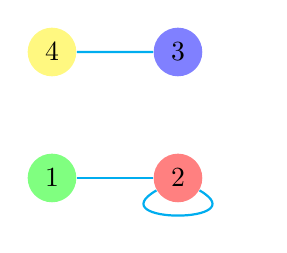
\begin{tikzpicture}
  [scale=.4,auto=left,every node/.style={circle}]
\node (n1)[fill=blue!50] at (4,4) {3};
  \node (n2)[fill=green!50] at (0,0)  {1};
  \node (n3)[fill=red!50] at (4,0)  {2};
  \node (n4)[fill=yellow!50] at (0,4)  {4};;
 \foreach \from/\to in {n3/n2,n1/n4}
    \draw[cyan,thick] (\from) -- (\to);
  \draw[cyan,thick]
  (n3) to[out=210,in=330,looseness=4] (n3);
\end{tikzpicture}
\caption{ Graph for Cube 1}\label{22g1}
\end{center}
\end{figure}

Similarly we can draw the graphs for each of the cubes Figures \ref{22g2}, \ref{22g3} and \ref{22g4}.

\begin{figure}[h]
\begin{center}
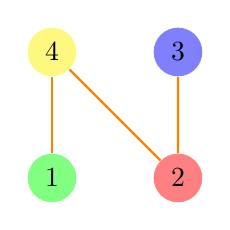
\begin{tikzpicture}
  [scale=.4,auto=left,every node/.style={circle}]
 \node (n1)[fill=blue!50] at (4,4) {3};
  \node (n2)[fill=green!50] at (0,0)  {1};
  \node (n3)[fill=red!50] at (4,0)  {2};
  \node (n4)[fill=yellow!50] at (0,4)  {4};

 \foreach \from/\to in {n3/n1,n3/n4,n2/n4}
    \draw[orange,thick] (\from) -- (\to);
\end{tikzpicture}
\caption{ Graph for Cube 2}\label{22g2}
\end{center}
\end{figure}

\begin{figure}[h]
\begin{center}
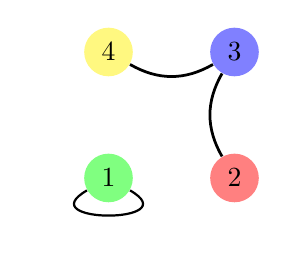
\begin{tikzpicture}
  [scale=.4,auto=left,every node/.style={circle}]
\node (n1)[fill=blue!50] at (4,4) {3};
  \node (n2)[fill=green!50] at (0,0)  {1};
  \node (n3)[fill=red!50] at (4,0)  {2};
  \node (n4)[fill=yellow!50] at (0,4)  {4};

 \path [line width=0.35mm,black] (n1) edge [bend right] (n3)
(n1) edge [bend left] (n4);
% \foreach \from/\to in {n3/n1,n1/n4}
%    \draw[black,thick] (\from) -- (\to);
     \draw[black,thick]
  (n2) to[out=210,in=330,looseness=4] (n2);
\end{tikzpicture}
\caption{ Graph for Cube 3}\label{22g3}
\end{center}
\end{figure}

\begin{figure}[h]
\begin{center}
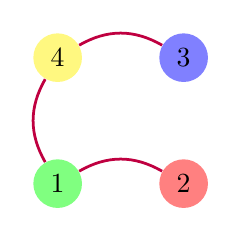
\begin{tikzpicture}
  [scale=.4,auto=left,every node/.style={circle}]
\node (n1)[fill=blue!50] at (4,4) {3};
  \node (n2)[fill=green!50] at (0,0)  {1};
  \node (n3)[fill=red!50] at (4,0)  {2};
  \node (n4)[fill=yellow!50] at (0,4)  {4};
 %\foreach \from/\to in {n3/n1,n1/n4,n2/n4}
 %   \draw[purple,thick] (\from) -- (\to);
 \path [line width=0.35mm, purple] (n2) edge [bend left] (n3)
(n1) edge [bend right] (n4)
(n2) edge [bend left] (n4);
\end{tikzpicture}
\caption{ Graph for Cube 4}\label{22g4}
\end{center}
\end{figure}

Now combining all these graphs in a single graph, we get a graph (looks complicated) Figure \ref{22g5}.

\begin{figure}[h]
\begin{center}
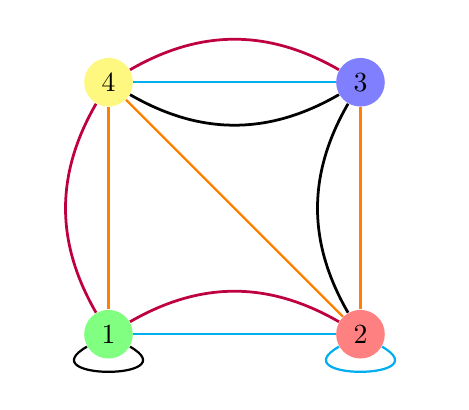
\begin{tikzpicture}
  [scale=.8,auto=left,every node/.style={circle}]
\node (n1)[fill=blue!50] at (4,4) {3};
  \node (n2)[fill=green!50] at (0,0)  {1};
  \node (n3)[fill=red!50] at (4,0)  {2};
  \node (n4)[fill=yellow!50] at (0,4)  {4};

 \foreach \from/\to in {n3/n2,n1/n4}
    \draw[cyan,thick] (\from) -- (\to);
  \draw[cyan,thick]
  (n3) to[out=210,in=330,looseness=4] (n3);
 \foreach \from/\to in {n3/n1,n3/n4,n2/n4}
    \draw[orange,thick] (\from) -- (\to); 
 \path [line width=0.35mm,black] (n1) edge [bend right] (n3)
(n1) edge [bend left] (n4);
     \draw[black,thick]
  (n2) to[out=210,in=330,looseness=4] (n2);  
   \path [line width=0.35mm, purple] (n2) edge [bend left] (n3)
(n1) edge [bend right] (n4)
(n2) edge [bend left] (n4);
\end{tikzpicture}
\caption{ Graph for all the cubes}\label{22g5}
\end{center}
\end{figure}

From this graph, we need to get which faces of the cubes are chosen as sides. Essentially there are four sides front and back, left and right (For this problem, top and bottom faces are not relevant.) The graph shown in Figure \ref{22g5} has this information as a subgraph. Let us try to get two subgraphs with orientation, so that we know the order of the sides. The first subgraph gives the front and back faces and the second subgraph gives the left and right faces.


The constraints on the subgraphs are
\begin{enumerate}
    \item The two subgraphs should have no edge in common; as an edge represents front to back or left to right. We cannot use them for both,
    \item Each subgraph should contain an edge from each cube (so that we use all the four cubes). In the graph this means all the edges should be different colors.
    \item The degree of each vertex should be two in the subgraph - that is colors cannot be repeated as per the problem statement.
    
\end{enumerate}

By examining the graph in Figure \ref{22g5}, we can get two subgraphs as follows Figures \ref{22g6} and  \ref{22g7}.

\begin{figure}[h]
\begin{center}
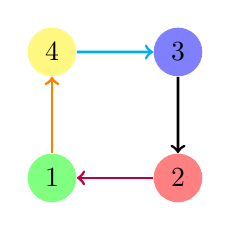
\begin{tikzpicture}
  [scale=.4,auto=left,every node/.style={circle}]
\node (n1)[fill=blue!50] at (4,4) {3};
  \node (n2)[fill=green!50] at (0,0)  {1};
  \node (n3)[fill=red!50] at (4,0)  {2};
  \node (n4)[fill=yellow!50] at (0,4)  {4};


 \path [line width=0.35mm,cyan] (n4) edge [->] (n1);
 
    \path [line width=0.35mm,orange] (n2) edge [->] (n4);
 \path [line width=0.35mm,black] (n1) edge [->] (n3);
 
   \path [line width=0.35mm, purple] (n3) edge [->] (n2);
;
\end{tikzpicture}
\caption{ Subgraph depicting front and back faces}\label{22g6}
\end{center}
\end{figure}

\begin{figure}[h]
\begin{center}
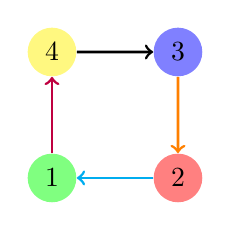
\begin{tikzpicture}
  [scale=.4,auto=left,every node/.style={circle}]
\node (n1)[fill=blue!50] at (4,4) {3};
  \node (n2)[fill=green!50] at (0,0)  {1};
  \node (n3)[fill=red!50] at (4,0)  {2};
  \node (n4)[fill=yellow!50] at (0,4)  {4};


 \path [line width=0.35mm,black] (n4) edge [->] (n1);
 
    \path [line width=0.35mm,purple] (n2) edge [->] (n4);
 \path [line width=0.35mm,orange] (n1) edge [->] (n3);
 
   \path [line width=0.35mm, cyan] (n3) edge [->] (n2);
;
\end{tikzpicture}
\caption{ Subgraph depicting left and right faces}\label{22g7}
\end{center}
\end{figure}

From Figures \ref{22g6} and \ref{22g7}, we can find out what the four sides are. 
The solution consists for each cube:
\begin{enumerate}
    \item Cube 1: front is yellow, back is blue, left is red, right is green (edge color is cyan in the subgraphs)
    \item Cube 2: front is green, back is yellow, left is blue, right is red (edge color is orange in the subgraphs)
    \item Cube 3: front is blue, back is red, left is yellow, right is blue (edge color is black in the subgraphs)
    \item Cube 4: front is red m back is green, left is green, right is yellow (edge color is purple in the subgrapgs)
    
\end{enumerate}

Ajur asked Rishnak how to find the subgraphs with the constraints he mentioned. Rishnak replied for the small case, one could do a visual inspection and get the decomposition. Otherwise it is a hard problem.

Ajur said suppose we have four cubes each cube colored in all faces with the same color. First cube is all red. Second Cube is all yellow. Third Cube is all blue and the fourth cube is all green. Then the two subgraphs will be easy (and of course the solution is trivial).

Graphs for all the four cubes is shown in Figure \ref{22g8}.
\tikzset{every loop/.style={min distance=10mm,looseness=10}}

\begin{figure}[h]
\begin{center}
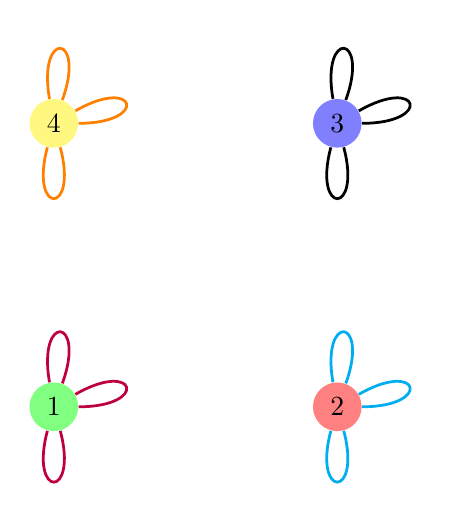
\begin{tikzpicture}
  [scale=.9,auto=left,every node/.style={circle}]
\node (n1)[fill=blue!50] at (4,4) {3};
  \node (n2)[fill=green!50] at (0,0)  {1};
  \node (n3)[fill=red!50] at (4,0)  {2};
  \node (n4)[fill=yellow!50] at (0,4)  {4};
 
 \path[line width=0.35mm, cyan] 
   (n3) edge [in=70,out=100,loop] (n3)
   (n3) edge  [in=0,out=30,loop] (n3)
   (n3) edge  [loop below] (n3); 
  \path[line width=0.35mm, orange] 
   (n4) edge [in=70,out=100,loop] (n4)
   (n4) edge  [in=0,out=30,loop] (n4)
   (n4) edge  [loop below] (n4); 
  \path[line width=0.35mm, black] 
   (n1) edge [in=70,out=100,loop] (n1)
   (n1) edge  [in=0,out=30,loop] (n1)
   (n1) edge  [loop below] (n1); 
  \path[line width=0.35mm, purple] 
   (n2) edge [in=70,out=100,loop] (n2)
   (n2) edge  [in=0,out=30,loop] (n2)
   (n2) edge  [loop below] (n2); 
   
\end{tikzpicture}
\caption{ Graph for all Cubes}\label{22g8}
\end{center}
\end{figure}

The decomposition into two subgraphs is shown in Figures \ref{22g9} and \ref{22g10}.
\begin{figure}[h]
\begin{center}
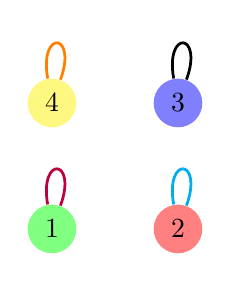
\begin{tikzpicture}
  [scale=.4,auto=left,every node/.style={circle}]
\node (n1)[fill=blue!50] at (4,4) {3};
  \node (n2)[fill=green!50] at (0,0)  {1};
  \node (n3)[fill=red!50] at (4,0)  {2};
  \node (n4)[fill=yellow!50] at (0,4)  {4};
 
 \path[line width=0.35mm, cyan] 
   (n3) edge [in=70,out=100,loop] (n3);
   
  \path[line width=0.35mm, orange] 
   (n4) edge [in=70,out=100,loop] (n4);
  
  \path[line width=0.35mm, black] 
   (n1) edge [in=70,out=100,loop] (n1);
  
  \path[line width=0.35mm, purple] 
   (n2) edge [in=70,out=100,loop] (n2);
    
   
\end{tikzpicture}
\caption{ Subgraph of front and back faces}\label{22g9}
\end{center}
\end{figure}
\begin{figure}[h]
\begin{center}
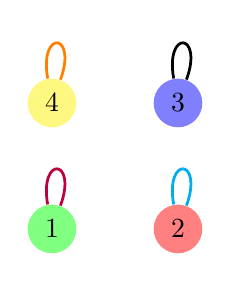
\begin{tikzpicture}
  [scale=.4,auto=left,every node/.style={circle}]
\node (n1)[fill=blue!50] at (4,4) {3};
  \node (n2)[fill=green!50] at (0,0)  {1};
  \node (n3)[fill=red!50] at (4,0)  {2};
  \node (n4)[fill=yellow!50] at (0,4)  {4};
 
 \path[line width=0.35mm, cyan] 
   (n3) edge [in=70,out=100,loop] (n3);
   
  \path[line width=0.35mm, orange] 
   (n4) edge [in=70,out=100,loop] (n4);
  
  \path[line width=0.35mm, black] 
   (n1) edge [in=70,out=100,loop] (n1);
  
  \path[line width=0.35mm, purple] 
   (n2) edge [in=70,out=100,loop] (n2);
    
   
\end{tikzpicture}
\caption{ Subgraph of left and right faces}\label{22g10}
\end{center}
\end{figure}

Ajur said that the solution is
\begin{enumerate}
    \item Cube 1: Front is red, back is red, left is red and right is red.
    \item Cube 2: Front is yellow, back is yellow, left is yellow and right is yellow.
    \item Cube 3: Front is blue, back is blue, left is blue and right is blue.
    \item Cube 4: Front is green, back is green, left is green and right is green.
\end{enumerate}

By this time, Ajur felt he had a clear understanding of all the concepts in graph theory. He thanked Rishnak for presenting him such interesting problems.

\textbf{Question for the twentieth day:} Rishnak asked Ajur how will you decompose the following graph for all New sets of cubes (He just drew the color of one face of one of the cubes) Figure \ref{22gq1}

\begin{figure}[h]
\begin{center}
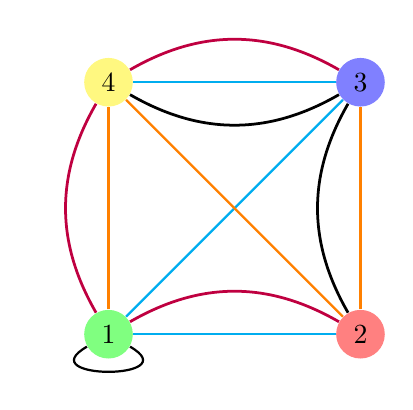
\begin{tikzpicture}
  [scale=.8,auto=left,every node/.style={circle}]
\node (n1)[fill=blue!50] at (4,4) {3};
  \node (n2)[fill=green!50] at (0,0)  {1};
  \node (n3)[fill=red!50] at (4,0)  {2};
  \node (n4)[fill=yellow!50] at (0,4)  {4};

 \foreach \from/\to in {n2/n1,n1/n4,n2/n3}
    \draw[cyan,thick] (\from) -- (\to);
 
 \foreach \from/\to in {n3/n1,n3/n4,n2/n4}
    \draw[orange,thick] (\from) -- (\to); 
 \path [line width=0.35mm,black] (n1) edge [bend right] (n3)
(n1) edge [bend left] (n4);
     \draw[black,thick]
  (n2) to[out=210,in=330,looseness=4] (n2);  
   \path [line width=0.35mm, purple] (n2) edge [bend left] (n3)
(n1) edge [bend right] (n4)
(n2) edge [bend left] (n4);
\end{tikzpicture}
\caption{ Graph for all the New cubes}\label{22gq1}
\end{center}
\end{figure}

\textbf{Answer:} Ajur was able to decompose the graphs (same as before!) \ref{22ga2} and \ref{22ga3}
\begin{figure}[h]
\begin{center}
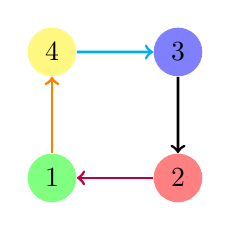
\begin{tikzpicture}
  [scale=.4,auto=left,every node/.style={circle}]
\node (n1)[fill=blue!50] at (4,4) {3};
  \node (n2)[fill=green!50] at (0,0)  {1};
  \node (n3)[fill=red!50] at (4,0)  {2};
  \node (n4)[fill=yellow!50] at (0,4)  {4};


 \path [line width=0.35mm,cyan] (n4) edge [->] (n1);
 
    \path [line width=0.35mm,orange] (n2) edge [->] (n4);
 \path [line width=0.35mm,black] (n1) edge [->] (n3);
 
   \path [line width=0.35mm, purple] (n3) edge [->] (n2);
;
\end{tikzpicture}
\caption{ Subgraph depicting front and back faces}\label{22ga2}
\end{center}
\end{figure}

\begin{figure}[h]
\begin{center}
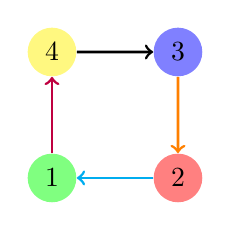
\begin{tikzpicture}
  [scale=.4,auto=left,every node/.style={circle}]
\node (n1)[fill=blue!50] at (4,4) {3};
  \node (n2)[fill=green!50] at (0,0)  {1};
  \node (n3)[fill=red!50] at (4,0)  {2};
  \node (n4)[fill=yellow!50] at (0,4)  {4};


 \path [line width=0.35mm,black] (n4) edge [->] (n1);
 
    \path [line width=0.35mm,purple] (n2) edge [->] (n4);
 \path [line width=0.35mm,orange] (n1) edge [->] (n3);
 
   \path [line width=0.35mm, cyan] (n3) edge [->] (n2);
;
\end{tikzpicture}
\caption{ Subgraph depicting left and right faces}\label{22ga3}
\end{center}
\end{figure}
Ajur and Jura bade good bye to Rishnak.  Kinaja was watching them from a distance. She smiled to herself that Ajur not only understood the concepts but also had the decency to thank Rishnak!